\documentclass[dvipdfmx, 9pt, a4paper]{jsarticle}
\usepackage[margin=15mm]{geometry}
\usepackage{fancyhdr}
\usepackage{multirow}
\usepackage{amsmath,  amssymb}
\usepackage{type1cm}
\usepackage{latexsym}
\usepackage{algorithmic}
\usepackage{algorithm}
\usepackage{ascmac}
\usepackage{listings,jvlisting}
\usepackage{tcolorbox}
\usepackage[utf8]{inputenc}
\usepackage{color}

\DeclareFixedFont{\ttb}{T1}{txtt}{bx}{n}{9}
\DeclareFixedFont{\ttm}{T1}{txtt}{m}{n}{9}
\definecolor{deepblue}{rgb}{0,0,0.5}
\definecolor{deepred}{rgb}{0.6,0,0}
\definecolor{deepgreen}{rgb}{0,0.5,0}

\renewcommand{\baselinestretch}{0.78}
\newcommand{\bm}[1]{{\mbox{\boldmath $#1$}}}
\newtheorem{Proof}{証明}
\def\qed{\hfill $\Box$}

\newcommand\pythonstyle{\lstset{
language=Python,
basicstyle=\ttm,
morekeywords={self},
keywordstyle=\ttb\color{deepblue},
emph={MyClass,__init__},
emphstyle=\ttb\color{deepred},
stringstyle=\color{deepgreen},
frame=tb,
showstringspaces=false
}}

\lstnewenvironment{python}[1][]
{
\pythonstyle
\lstset{#1}
}
{}

\newcommand\pythonexternal[2][]{{
\pythonstyle
\lstinputlisting[#1]{#2}}}
\newcommand\pythoninline[1]{{\pythonstyle\lstinline!#1!}}


\begin{document}
\begin{center}
{\fontsize{18pt}{1pt}\selectfont フーリエ変換とラプラス変換}\\
\end{center}

\section*{はじめに}
\begin{figure}[b]
\begin{center}
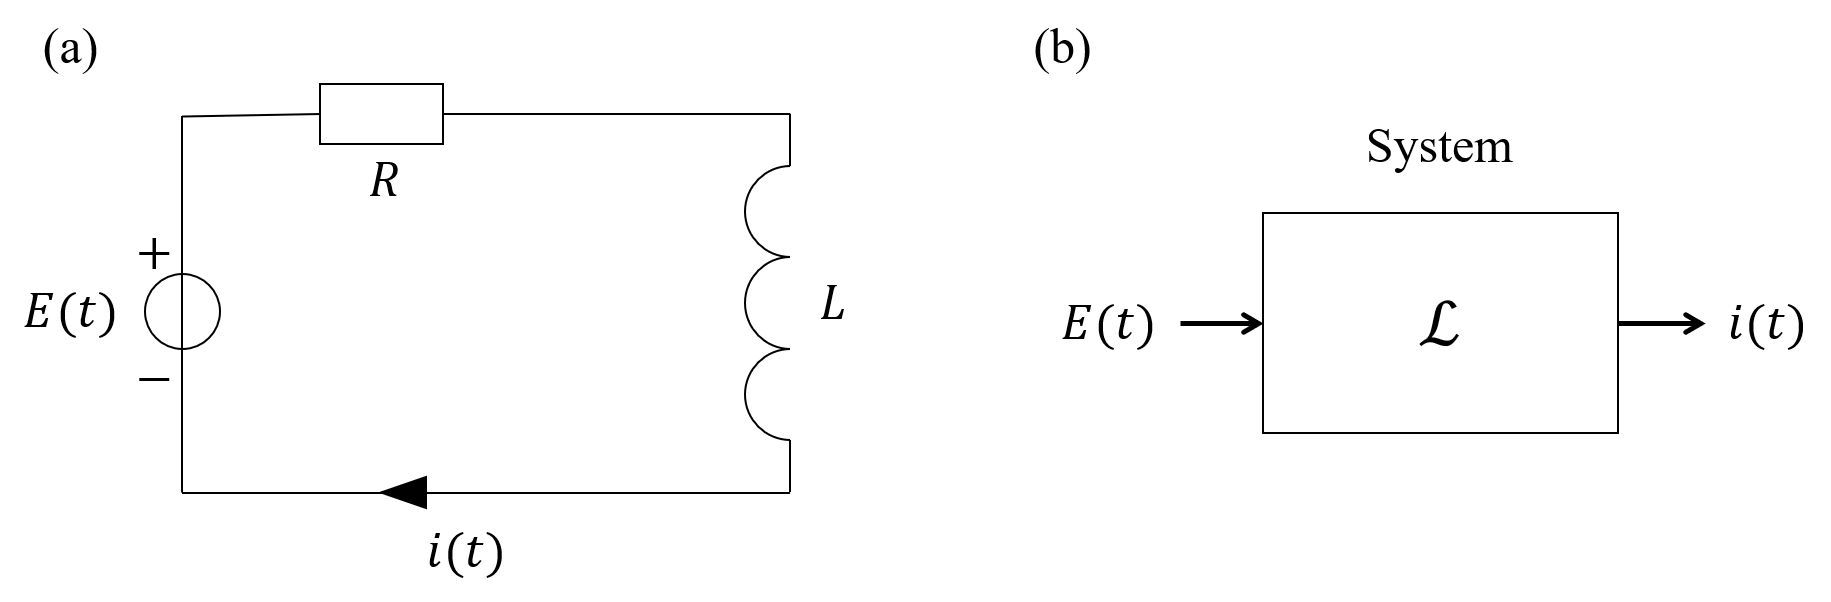
\includegraphics[width=10cm]{fig1.png}
\caption{(a)電気回路の例(b)システムとしての描像}
\end{center}
\end{figure}
当然ながら物理と数学の関係は深く、「物理の言語は数学である」と言うこともできる。物理モデルと数学モデルという言葉があるが、ここでは抽象的な物理モデルを数式化したものが数学モデルと定義しよう。例えば、図1(a)のような電気回路を用いて印加電圧と電流のデータを得たとする。この実在現象からキルヒホッフの法則を導くことができたとき、この問題は晴れて抽象化され、物理モデルを得られたことになる。これに対して数学モデルは、キルヒホッフの法則を時間の偏微分方程式に変換することで得られる。明らかに数学モデルの方が科学として扱いやすい。\par
異なる物理現象の数学モデルが類似している場合、互いの物理現象にも類似性があることに気付く。例えば電気回路とバネ振動は数理モデル上類似している。この気付きは物理モデルだけからだと得づらいだろう。数理モデルが類似している場合、その数理モデルを解明するだけで両物理モデルを解明したことになる。それゆえ物理の問題であっても、物理モデルから離れて数学モデルのみで議論することも多い。\par
数学モデルのみで考えるならば、その現象がどのような物理系で構成されているかに興味が薄れる。例えば偏微分方程式が所与であれば、それを構成する電気回路の詳細な図は不要になる。従って数学モデルで考えるときは図1(b)のように$\mathcal{L}$と書かれたボックスで略記してしまう。このような物理系に対応するものを、信号処理の分野ではシステムと呼ぶ。なお、システムを$\mathcal{L}$と書いたのは、システムが線形性を満たすためである。\par
図1(b)にはシステム以外に印加電圧と電流も表記されている。これらは時間の関数で、それぞれ入力および出力と言う。つまり、このシステムは入力が所与のときにどのような出力が得られるかを考えていることになる。なお、信号処理の問題では入出力のことを信号と呼んでいる。\par
さて、本資料の主題はフーリエ変換とラプラス変換であるが、これらは線形な物理モデルに対応する数学モデルでよく用いられる。例えば時系列波形を入出力として扱うとき、それらを時間領域よりも周波数領域の方が見通しやすいためである。フーリエ変換とラプラス変換に関する書籍は数多くあるが、両方を一気通貫して説明したものは驚くほど少ない。また、フーリエ変換とラプラス変換を信号処理におけるツールとして見るあまり、数学的厳密さを欠いた書籍が多いことも残念に思う。本資料では、フーリエ変換とラプラス変換の関連性を議論し、できるだけ数学的にも深堀するよう試みた。

\section{前準備}
\subsection{システムの諸定義}
\subsubsection{線形時不変システム(LTシステム)}
\begin{tcolorbox}[title=線形システム]
 入力$u$と$v$に対して$\mathcal{L}(au+bv)=a\mathcal{L}(u)+b\mathcal{L}(b)$が成立するとき、このシステムは線形であると言う。
\end{tcolorbox}
\begin{tcolorbox}[title=時不変システム]
 入力$u(t)$に対応する出力が$v(t)$であるとする。任意のスカラー$t_0$に対して入力$u(t-t_0)$の出力が$y(t-t_0)$となるとき、このシステムは時不変であると言う。
\end{tcolorbox}
線形かつ時不変なシステムのことをLTシステムと書くことが多い。フーリエ変換とラプラス変換はLTシステムにおいて非常に重要な役割を担う。以下はLTシステムで成立する定理である。
\begin{itembox}[l]{定理1.1}
 LTシステムに時間調和関数$u(t)=ce^{i\omega t}$を入力したとする($c \in \mathbb{C}$、$\omega \in \mathbb{R}$)。このときの出力$v(t)$も同じ周波数の時間調和関数になる。
\end{itembox}
{\bf 証明}:時不変であるため
\begin{equation}
v(t-\tau)=\mathcal{L}(u(t-\tau))=ce^{-i\omega \tau}\mathcal{L}(u(t))=ce^{-i\omega \tau}v(t) \notag
\end{equation}
が任意の$\tau$で成立する。上式で$t=0$かつ$\tau=-t$としたとき、$v(t)=v(0)e^{i\omega t}$となるため、出力も同じ周波数の時間調和関数になることが確認できた。\qed \par
定理1.1より、入力$e^{i\omega t}$に対するLTシステムの出力は$H(\omega)e^{i\omega t}$と書くことができる。ここで$H(\omega) \in \mathbb{C}$であり、周波数応答と言う。定理1.1の証明時に確認したように、周波数応答は周波数にのみ依存する。$H(\omega)$が$|H(\omega)|e^{i\Phi(\omega)}$のように書き換えられるとき、$|H(\omega)|$を振幅応答、$\Phi(\omega)$を位相応答と言う。

\subsubsection{安定システム}
\begin{tcolorbox}[title=有界信号]
 信号$u(t) \in \mathbb{C}$を考える。任意の$t$に対して$|u(t)| \leq K$を満たす実数$K$が存在するとき、信号は有界であると言う。
\end{tcolorbox}
\begin{tcolorbox}[title=安定システム]
 任意の有界信号な入力に対応する出力も有界であるとき、このシステムは安定であると言う。
\end{tcolorbox}
安定でないシステムの代表例は非減衰の自由振動であろう。入力を加振力、出力を速度としたとき、加振力の周波数が固有振動数ならば速度は発散する。このような物理現象を共鳴と言い、数学モデルでは時に解無しと見なす。

\subsubsection{因果性システム}
物理系では当然だが、ある時刻$t_0$の出力$v(t_0)$が$t<t_0$の入力$u(t)$にのみ依存するとき、そのようなシステムを因果性システムと言う。以下は因果性システムの厳密な定義である。
\begin{tcolorbox}[title=因果性システム]
 ある時刻$t_0$に対し、$u(t)=v(t)~(t<t_0)$な2つの信号を考える。任意の時刻$t(<t_0)$に対して、$\mathcal{L}(u)=\mathcal{L}(v)$が成立するならば、このシステムのことを因果性システムと言う。
\end{tcolorbox}

\subsection{数学の準備}
\subsubsection{多項関数}
後述するように、ラプラス変換では複素多項関数$P(z)=\sum_{i=0}^n a_iz^i$を考えることが多い。ここで$a_n, z \in \mathbb{C}$かつ$a_n \neq 0$であり、これを$n$次多項関数と言う。代数学によると、$P(z)$は
\begin{equation}
P(z)=a_n(z-z_1)^{\nu_1}...(z-z_k)^{\nu_k} \notag
\end{equation}
のように分解することができる。なお$\nu$のことを重複度と言い、$\sum \nu_i=n$を満たす。\par
ラプラス変換で見られる多項関数の係数は、実数であることが多い。以下はその際に重要な命題である。
\begin{itembox}[l]{命題1.1}
 多項式の係数が実数の場合、$\alpha$が解ならばその共役$\bar{\alpha}$も解である。
\end{itembox}
{\bf 証明}:$P(\alpha)=0$のとき、$\overline{P(\alpha)}=0$が成立するが、これは
\begin{equation}
\overline{P(\alpha)}=\sum a_i \overline{\alpha}^i=P(\overline{\alpha})=0 \notag
\end{equation}
であるため、命題1.1は正しい。\qed
\begin{itembox}[l]{命題1.2}
 多項関数の係数が実数の場合、多項関数は実係数の一次多項関数と二次多項関数を用いて分解できる。
\end{itembox}
{\bf 証明}:前述の通り、$P(z)=\sum a_iz^i$は$a_n(z-z_1)^{\nu_1}...(z-z_k)^{\nu_k}$のように一次多項関数で分解できる。このうち$z_i$が複素数だとした場合、$\overline{z_i}$も$P(z)=0$の解となる。従って適当な多項関数$Q(z)$を用いて、$P(z)=(z-z_i)(z-\overline{z_i})Q(z)$のように分解することができる。すると、
\begin{equation}
(z-z_i)(z-\overline{z_i})=(z^2-2{\rm Re}(z_i)z+|z_i|^2) \notag
\end{equation}
より、これは実係数の二次多項関数だと分かる。以上より命題1.2は正しい。\qed \par
実係数の多項式で最も重要なのは$z^n=1$だろう。$z=Ae^{i\theta}$としたとき、$z^n=A^ne^{in\theta}$であるため、この解は
\begin{equation}
z_k=e^{i2k\pi/n}={\rm cos}\left(\frac{2k\pi}{n}\right)+i{\rm sin}\left(\frac{2k\pi}{n}\right)~~~{\rm for}~k=0,1,...,n-1 \notag
\end{equation}
だと直ぐにわかる。

\subsubsection{部分分数展開}
ラプラス変換では下記のような有理関数
\begin{equation}
F(z)=\frac{P(z)}{Q(z)}=\frac{a_nz^n+...+a_1z+a_0}{b_mz^m+...+b_1z+b_0}~~~~a,~b \in \mathbb{R}
\end{equation}
を考えることが多い。分母の$Q(z)$のことを特別に特性多項式と呼ぶ。また、特性多項式がゼロとなる$z \in \mathbb{C}$のことを根と言う。$F(z)$の根が$\{ z_1, ..., z_k\}$であるとき、$Q(z)=b_n(z-z_1)^{\nu_1}...(z-z_k)^{\nu_k}$のように分解できることは前述の通りである。\par
厳密さを欠いた表現ではあるが、部分分数展開は「式(1)のような有理関数をより単純な有理関数の和に変換する手法」と言える。こうすることのご利益はラプラス変換の章に譲るとして、今はそのテクニックのみ議論しよう。なお、式(1)の次数に関して$n<m$を仮定する。これは、$n\geq m$ならば$F(z)=D(z)+R(z)/Q(z)$のように分解することができ、新しい有理関数$R(z)/Q(z)$は特性多項式の次数の方が大きくなるためである。とにかく、今は$n<m$な有理関数で議論したい。\par
ラプラス変換の書籍は数多くあるが、部分分数展開の議論はあまり統一されておらず、主に2種類の結果を是としている。まず初めに比較的単純な方法を紹介する。
\begin{tcolorbox}[title=部分分数展開(係数が複素数となり得る方法)]
式(1)の有理関数について考える(ただし$n<m$)。特性多項式が$Q(z)=b_n(z-z_1)^{\nu_1}...(z-z_k)^{\nu_k}$のように分解できる場合、$F(z)$は
\begin{equation}
F(z)=\sum_{i=1}^k\sum_{j=1}^{\nu_i}\frac{c_{ij}}{(z-z_i)^j}~~~~c_{ij} \in \mathbb{C}
\end{equation}
のように部分分数展開できる。
\end{tcolorbox}
この場合の分子は必ず定数であり、分母は線形もしくは線形な多項関数の整数乗となる。部分分数展開の処理は定数$c_{ij}$の導出と言えるが、これは式(2)右辺の有理関数を通分して係数比較することで求まる。\par
有理関数の根$\{ z_1, ..., z_k\}$が実数である場合、部分分数展開の結果も実係数な有理関数で構成されることになる($c_{ij}$も実数となることは明らか)。後ほど気付くように実係数な有理関数はラプラス変換において扱いやすいので、この特性は望ましい。したがって式(2)の部分分数展開で面倒になるのは、根に複素数が含まれる場合である。\par
それでは次に、根に複素数が含まれているときでも実係数の有理関数で部分分数展開する方法を議論しよう。命題1.2より、実係数の複素多項式は実係数な1次多項式と2次多項式で分解できる。そこで同じ$Q(z)$が
\begin{equation}
Q(z)=b_m(z-z_1)^{\nu_1}...(z-z_p)^{\nu_p}(z^2-2{\rm Re}(z_{p+1})z+|z_{p+1}|^2)^{\nu_{p+1}}...(z^2-2{\rm Re}(z_k)z+|z_k|^2)^{\nu_k}
\end{equation}
のようにも分解できるとする。このとき、以下の部分分数展開も考えられる。
\begin{tcolorbox}[title=部分分数展開(係数も実数となる方法)]
式(1)の有理関数について考える(ただし$n<m$)。特性多項式が式(3)のように分解できる場合、$F(z)$は
\begin{equation}
F(z)=\sum_{i=1}^p\sum_{j=1}^{\nu_i}\frac{c_{ij}}{(z-z_i)^j}+\sum_{i=p+1}^k\sum_{j=1}^{\nu_i}\frac{d_{ij}z+e_{ij}}{(z^2-2{\rm Re}(z_i)z+|z_i|^2)^j}~~~~c_{ij},~d_{ij},~e_{ij} \in \mathbb{R}
\end{equation}
のように部分分数展開できる。
\end{tcolorbox}
式(2)と違い式(4)は実係数な有理関数で展開できているため、その分ラプラス変換では扱いやすかったりする(後述)。

\subsubsection{区分的連続}
物理学(特にCAE)の議論をしていると、関数の連続性や微分可能特性の確認が疎かになりがちである。例えば極限値$f(t-)={\rm lim}_{h \to 0}f(t-h)$や$f(t+)={\rm lim}_{h \to 0}f(t+h)$などの区別を特に意識しなかったりする。しかしながら、フーリエ変換やラプラス変換の議論ではあまりずぼらになってはいけない。本項では関数の諸定義を紹介する。\par
\begin{tcolorbox}[title=区分的連続関数(piecewise continuous function)]
区間$[a, b]$において関数$f(t)$が以下の条件を満たすとき、$f(t)$は$[a, b]$において区分的連続であると言う。
\begin{itemize}
\item $(a, b)$において不連続な点$\{ t_1, ..., t_n \}$が有限個しか存在しない。
\item $f(a+)$、$f(b-)$、$f(t_i+)$、$f(t_i-)$が存在する。
\end{itemize}
また、区間が実数全体である場合は単に「区分的連続」と言う。
\end{tcolorbox}
\begin{figure}[t]
\begin{center}
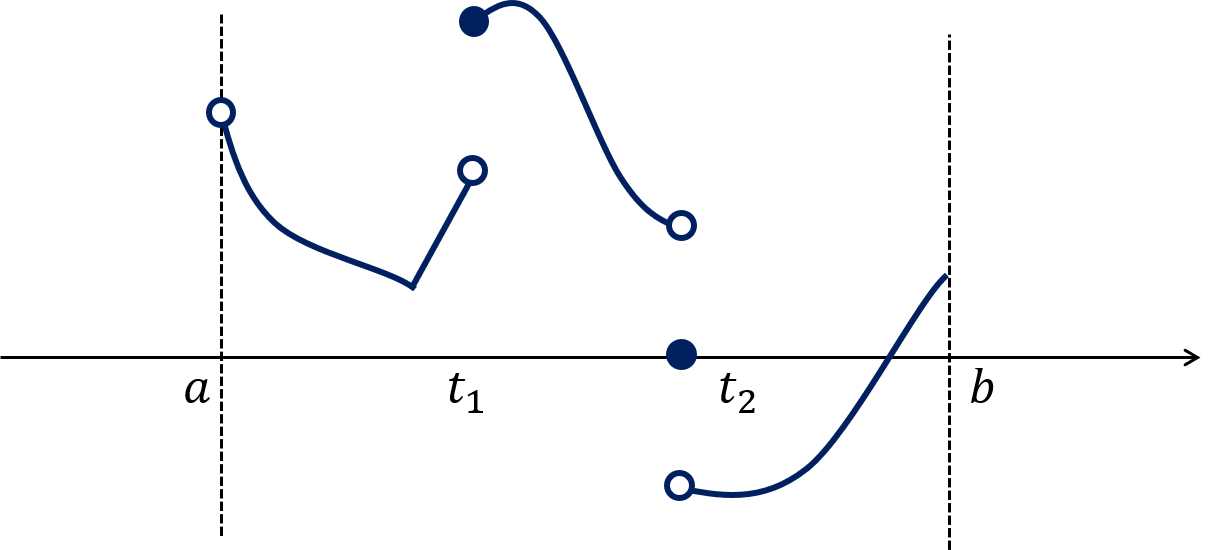
\includegraphics[width=10cm]{fig2.png}
\caption{区分的連続関数の例}
\end{center}
\end{figure}
図2に区分的連続関数の例を示す。個人的に区分的連続性を満たさない関数を見つけることの方が難しいと感じている。何とか絞りだせた区分的連続でない例が$f(t)={\rm sin}(1/t)$である。これは$t=0$において区分的連続性の条件に反する。\par
区分的連続関数$f(t)$の導関数$f'(t)$も区分的連続性を満たすとき、この関数のことを区分的に滑らかな関数(piecewise smooth function)と言う。導関数$f'(t)$に関しても$f'(t-)$や$f'(t+)$といった値を定められるが、一方で以下のような値
\begin{equation}
f'_+(t)={\rm lim}_{h \to 0}\frac{f(t+h)-f(t+)}{h},~~~f'_-(t)={\rm lim}_{h \to 0}\frac{f(t+h)-f(t-)}{h} \notag
\end{equation}
も定められる(これらを右導関数および左導関数と言う)。多くの場合$f'(t+)=f'_+(t)$や$f'(t-)=f'_-(t)$が成り立つが、区分的連続関数でも以下の定理が言える。
\begin{itembox}[l]{定理1.2}
関数$f(t)$が$[a,b]$において区分的滑らかであるとき、$f'(a+)=f'_+(a)$、$f'(b-)=f'_-(b)$が成り立つ。また、任意の$t(a<t<b)$において$f'(t+)=f'_+(t)$、$f'(t-)=f'_-(t)$が成り立つ。
\end{itembox}\par
区分的連続関数の積分が定義されているとき、以下の定理が成立する。
\begin{itembox}[l]{定理1.3}
$f(t)$は$[a,b]$において区分的連続であるとする。任意の$x \in [a,b]$に対して$F(x)=\int_a^xf(t)dt$を定義したとき、この$F$は区分的に滑らかである。
\end{itembox}

\subsubsection{周期関数}
任意の$t$に対して$f(t+T)=f(t)$となるような$T \in \mathbb{R}$が存在するとき、$f(t)$は周期$T$の周期関数と言う。明らかに$f(t)$が周期$T$の周期関数であれば、任意の自然数$n$に対して$nT$の周期関数であることも同時に成り立つ。周期$T$に対して$\omega_0=2\pi/T$のことを基本周波数と言う。
\begin{itembox}[l]{命題1.3}
$f(t)$は周期$T$の周期関数とする。このとき任意の$\tau$に対して$\int_{-T/2}^{T/2}f(t)dt=\int_{-T/2+\tau}^{T/2+\tau}f(t)dt$が成立する。
\end{itembox}\par
これは、周期関数の1周期分の積分は選択した時間領域に依存しないことを意味している。\par
周期関数の最も有名な例として三角関数($A{\rm sin}(n\omega_0t+\phi)$及び$A{\rm cos}(n\omega_0t+\phi)$)がある。また、それぞれに対応可能な複素関数$ce^{in\omega_0t}$も有名であろう。ここで$c$は複素数であり、$c=Ae^{i\phi t}$である。物理的に考えれば周期とは正の実数であるべきで、それゆえ周波数も正の実数になるが、数学的には負の周波数も認められる。図3の複素平面で考えたとき、正の周波数は反時計回りに、負の周波数は時計周りに移動することが分かる。ただし物理現象として観測されるのは実部もしくは虚部の一方であるため、結果的に得られる信号は周波数$|\omega_0|$に統一できる。

\begin{figure}[b]
\begin{center}
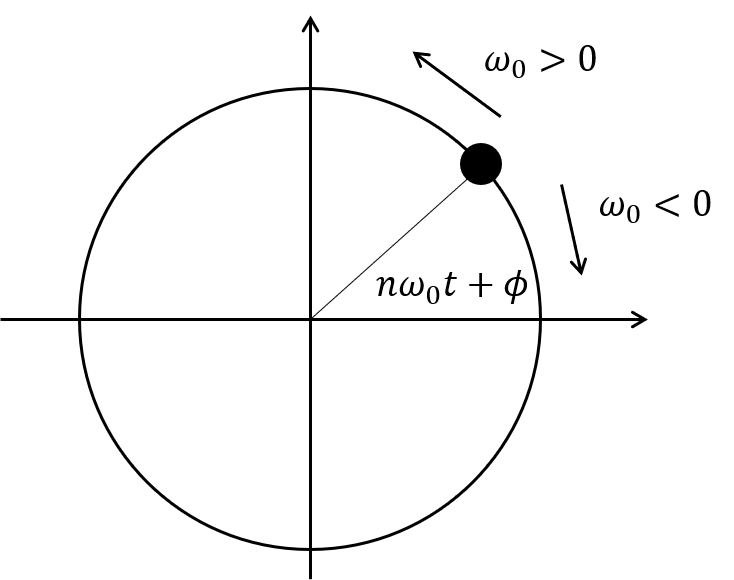
\includegraphics[width=6cm]{fig3.png}
\caption{正の周波数と負の周波数の概念図}
\end{center}
\end{figure}

\subsubsection{三角関数系}
フーリエ級数を理解する上で最も重要なのが三角関数系なる概念である。区間$[-T/2, T/2]$で定義された関数を全て含む集合$V$を考える。$V$は明らかに次元数が無限のベクトル空間である。$V$の直交基底として$\{{\rm cos}n\omega_0t, {\rm sin}m\omega_0t~|~n=0,1,...~~m=1,2,...\}$が知られており($\omega_0=2\pi/T$)、これを三角関数系と言う。なお、周期$T$の周期関数を全て含む集合は$V$と等しい。従って三角関数系は周期$T$の周期関数を全て含む集合の基底でもある。\par
任意のベクトル${\rm cos}n\omega_0t({\rm sin}m\omega_0t)$に関して、$\int_{-T/2}^{T/2}{\rm cos}n\omega_0tdt(\int_{-T/2}^{T/2}{\rm sin}m\omega_0tdt)=0$が成立する。また、三角関数系が直交基底であることは以下の式より確認できる。
\begin{equation}
\int_{-T/2}^{T/2}{\rm cos}n\omega_0t \cdot {\rm cos}m\omega_0t=
\left\{
\begin{array}{ll}
0 & n \neq m \\
T/2 & n=m \neq 0 \\
T & n=m=0
\end{array}\right. \notag
\end{equation}
\begin{equation}
\int_{-T/2}^{T/2}{\rm sin}n\omega_0t \cdot {\rm sin}m\omega_0t=
\left\{
\begin{array}{ll}
0 & n \neq m \\
T/2 & n=m \\
\end{array}\right. \notag
\end{equation}
\begin{equation}
\int_{-T/2}^{T/2}{\rm cos}n\omega_0t \cdot {\rm sin}m\omega_0t=0 \notag
\end{equation}


\subsubsection{数列と級数}
数列とは、その名の通り数を列にして定義されたものである。本資料では数列を$(a_n)\{n=0,1,2,...\}$のように書くことにする。また数列を成す数値$a_n$は、特に断りがなければ複素数とする。一般的に$n$の値は限りなく大きくすることができ、それゆえ$a_n$の極限値${\rm lim}_{n\to \infty}a_n$も定義される。$a_n$が$a$に収束するとは、${\rm lim}_{n \to \infty}|a_n-a|=0$を満たすような$a$が存在することを言う。ここで$|a_n-a|$は複素平面上、つまり2次元空間上での距離であり、高等数学で学んだ実数列の収束から微妙に拡張されている。また、数列が収束しない場合、その数列は発散すると言う。\par
数列$(a_n)$に対して$s_n=\sum_{i=0}^na_i$のことを数列の部分和と言う。また、$s_n$の極限値$s={\rm lim}_{n \to \infty}s_n$のことを級数と言う。明らかに$(a_n)$が収束するときに限り$s_n$も収束する。
\begin{itembox}[l]{定理1.4}
級数$\sum_{n=0}^\infty a_n$が収束するならば、${\rm lim}_{n \to \infty}a_n=0$が成立する。
\end{itembox}
{\bf 証明}:$\sum_{n=0}^\infty a_n$は$s$に収束するとする。このとき、
\begin{equation}
{\rm lim}_{n \to \infty}a_n={\rm lim}_{n \to \infty}(s_n-s_{n-1})={\rm lim}_{n \to \infty} s_n - {\rm lim}_{n \to \infty} s_{n-1}=s-s=0 \notag
\end{equation}
より、確かに$(a_n)$はゼロに収束する。\qed
\begin{itembox}[l]{命題1.4}
数列$(a_n)$に対して$L={\rm lim}_{n \to \infty}|a_{n+1}/a_n|$を定義する。
\begin{itemize}
\item $L<1$ならば$(a_n)$は絶対収束する。
\item $L>1$ならば$(a_n)$は発散する。
\item $L=1$のときは、これだけではどちらとも言えない。
\end{itemize}
\end{itembox}
定理1.4は必要十分条件でないことに注意してほしい。数列がゼロに収束するにも関わらず級数が収束しない例として調和級数$\sum_{n=0}^\infty (1/n^p)$がある。ここで$p$は正の定数である。
\begin{itembox}[l]{命題1.5}
$p>1$のとき、調和級数は収束し、$0<p \leq 1$のとき発散する。
\end{itembox}
{\bf 証明}:数値計算における積分の様子を想像すると、$\int_1^{n+1}(1/x^p)dx \leq \sum_{i=0}^n(1/i^p) \leq \int_0^n(1/x^p)dx$であることに気付き、
\begin{equation}
\frac{(n+1)^{1-p}-1}{1-p} \leq \sum_{i=0}^n(1/i^p) \leq \frac{n^{1-p}}{1-p} \notag 
\end{equation}
なる関係が得られる。上式に対して$n \to \infty$とすれば、確かに命題は正しい。\qed \par
\begin{tcolorbox}[title=絶対収束]
級数$s=\sum_{n=0}^\infty a_n$に関して、$\sum_{n=0}^\infty |a_n|$がある値に収束するならば、この級数は絶対収束すると言う。
\end{tcolorbox}
\begin{itembox}[l]{命題1.6}
複素数列$(a_n)$に対して、${\rm Re}(a_n)=u_n$、${\rm Im}(a_n)=v_n$とする。$(a_n)$が絶対収束する必要十分条件は、$(u_n)$および$(v_n)$が絶対収束することである。
\end{itembox}
\begin{itembox}[l]{定理1.6}
絶対収束する数列は収束する。
\end{itembox}

\subsubsection{幾何数列}
最も有名な数列の一つに幾何数列というものがあり、それは$\{ 1, z, z^2, z^3, ...\}(z \in \mathbb{C})$で定義されている。幾何数列の部分和を$s_n=\sum_{i=0}^nz^i$、幾何級数を$s$と書き表そう。$z=1$のとき$s_n=1+n$であるため、この幾何級数は発散する。一方で$z \neq 1$であるとき、$s_n-zs_n=(1-z)s_n=1-z^{n+1}$であるため$s_n=(1-z^{n+1})/(1-z)$だとわかる。従って、$|z| \geq 1$のとき幾何級数は発散し、$|z| < 1$のとき$s=1/(1-z)$に収束する(絶対収束することも明らかである)。

\subsubsection{関数列と関数項級数}
関数列とは定義域を共有した無限個の関数の列のことであり、例えばフーリエ級数で登場する概念である。関数列に対して、$\sum_{n=0}^\infty f_n(t)$なる和を考えることもできる。この値は当然ながら$t$の値に依存するし、収束するか否かも$t$次第である。定義域における任意の$t$に対してこの和が収束するとき、これを新しい関数$f(t)=\sum_{n=0}^\infty f_n(t)$として書くことができる。この関数$f(t)$のことを関数列の各点収束という。\par
定義より各点収束の導関数は$f'(t)=\sum_{n=0}^\infty f'_n(t)$となる。ほとんどの場合は各点収束の導関数の導出時に注意を要さないが、厄介な特性を持つ関数が存在することも確かである。ごくまれに任意の$f_n(t)$が微分可能であるにも関わらず$f(t)$は微分不可能なんてことがある。例として$f_n(t)={\rm sin}(nt)/n^2$を考えてみよう。この導関数は$f'_n(t)={\rm cos}(nt)/n$であるため、$t=0$のとき$f'(t)=\sum_{n=0}^\infty 1/n$となる。これは正に$p=1$の調和級数であり、発散することは既に確かめた。\par
各点収束の積分でも注意しなければならない。ほとんどの場合は$\int f(t)dt=\int \sum_{n=0}^\infty f_n(t)dt=\sum_{n=0}^\infty \int f_n(t)dt$が成立するが、ときに最右辺の等式が成立しないこともある(その例の紹介は他書に譲る)。\par
上記のような導関数や積分の議論を続けるには、一様収束なる概念を導入しなければならない。しかしながらこれは本書の範疇を超えるため、これ以上の議論は控える。そもそも、物理学で登場する関数はあまり特殊でないと思える。そこで本資料ではあまり難しく考えずに、下記2式はいつも成り立つと仮定することにする。
\begin{equation}
f'(t)=\sum_{n=0}^\infty f'_n(t),~~~\int f(t)dt=\int \sum_{n=0}^\infty f_n(t)dt=\sum_{n=0}^\infty \int f_n(t)dt \notag
\end{equation}

\subsubsection{べき級数}
$\sum_{n=0}^\infty c_nz^n$のような形で定義される級数のことを特別にべき級数と言う($c_n, z \in \mathbb{C}$)。前述の幾何級数はべき級数の一例と言える。べき級数が収束する$z$の集合(例えば幾何級数なら$\{z |~~|z| < 1\}$)を定義域とした場合、べき級数は関数列$f_n(z)=c_nz^n$に対する各点収束と言える。ただし、当然ながらべき級数が発散する$z$において各点収束は定義できない。\par
べき級数の場合、命題1.4の$L$は$L={\rm lim}_{n \to \infty}|c_{n+1}/c_n||z|$となる。従ってべき級数が絶対収束する条件は
\begin{equation}
|z| < \left|\frac{c_{n+1}}{c_n}\right|=R \notag
\end{equation}
と書ける。つまり複素平面上の「中心が原点で半径が$R$な円内」であればべき級数は収束すると分かる(なお$z=0$においてはべき級数は必ず収束する。場合によっては$R=0$となるが、それでも$z=0$は上式の例外であることに注意)。このような円を収束円と言い、上式の$R$を収束半径と言う。\par
収束円内に限れば、数列を$f_n(z)=c_nz^n$の関数列と見なし、べき級数を$f(z)=\sum_{n=0}^\infty f_n(z)$の各点収束と考えることができる。実関数ではあるが、テイラー展開はべき級数を各点収束と見なした分かりやすい例である。

\section{フーリエ級数}
本章ではフーリエ級数について議論する。フーリエ級数は線形システムを扱う分野でよく利用されるが、その数学的理論は驚くほど難しい。そこでまずは肩慣らしのために、フーリエ級数の基礎と題して感覚的な解釈を紹介する。ある程度印象をつかめた後にフーリエ級数に関する定理に踏み込む。
\subsection{フーリエ級数の基礎}
\subsubsection{はじめに}
定常的に動き続ける機械や毎年のように観測できる自然現象など、私たちの周りは周期的な現象であふれている。この周期的な現象を関数$f(t)$で表すことができ、かつ$f(t)$が何か関数列の各点収束であったとする。本章の本質は関数列に三角関数を採用し、周期関数を
\begin{equation}
f(t)=\frac{a_0}{2}+\sum_{n=1}^\infty (a_n{\rm cos}n\omega_0t+b_n{\rm sin}n\omega_0t)
\end{equation}
のような各点収束で表そうとすることにある(ここで$A \in \mathbb{R}$は定数。また$f(t)$の周期を$T$としたとき、$\omega_0=2\pi/T \in \mathbb{R}$。後ほど議論するが、上式の等式が成立しないこともあるので注意)。なお、物理に関する観測値は$\mathbb{R}$に含まれるので、特に断りがなければ本資料で扱う関数も実関数とする。$f(t)$に対する上式の右辺のような変換をフーリエ級数と言い、$a_n, b_n \in \mathbb{R}$のことをフーリエ係数と言う。\par
対称のシステムが線形であり、かつ入力が上式のように表せたとする。このとき、システムの出力は${\rm cos}n\omega_0t$や${\rm sin}n\omega_0t$における出力の線形和で表せることは前述した通りである。そのため、フーリエ級数を利用した線形システムの解析では、これら三角関数に対する応答が肝と言える。フーリエ級数の議論では、この応答とフーリエ係数の計算方法が主役となる。

\subsubsection{フーリエ係数とフーリエ級数}
フーリエ係数は三角関数系の直交性を利用すれば求められる。例えば$a_n$を求めたいのであれば$f(t)$と${\rm cos}n\omega_0t$の内積から簡単に導出できる。フーリエ係数について以下に纏めた。
\begin{tcolorbox}[title=フーリエ係数]
周期$T$の周期関数$f(t)$に関して、
\begin{equation}
a_n=\frac{2}{T}\int_{-T/2}^{T/2}f(t)\cdot {\rm cos}n\omega_0t dt~~~n=0,1,2,... \notag
\end{equation}
\begin{equation}
b_n=\frac{2}{T}\int_{-T/2}^{T/2}f(t)\cdot {\rm sin}n\omega_0t dt~~~n=1,2,... \notag
\end{equation}
が定義できる場合、これらをフーリエ係数と言う。
\end{tcolorbox}
なお、上式では積分域を$[-T/2,T/2]$と定義したが、積分区間が$T$であれば結果が同様であることは命題1.3の通りである。もちろんこの積分が定義できないのであれば、フーリエ係数も得られない訳であるが、その辺りは次節で議論する。
\begin{tcolorbox}[title=フーリエ級数]
周期$T$の周期関数$f(t)$に関して、フーリエ係数が得られた場合、$a_0/2+\sum_{n=1}^\infty(a_n{\rm cos}n\omega_0t+b_n{\rm sin}n\omega_0t)$のことをフーリエ級数と言う。
\end{tcolorbox}
式(5)と違い$f(t)$とフーリエ級数を等式で結んでいないことに注意してほしい。多くの場合、両者の等号は成立するが、成立しないこともある。従って式(5)は正しくない訳であり、それゆえ「各点収束で表そうとすることにある」と回りくどい言い方をしていた。例えば$f(t)$が有界な信号であったとしてもフーリエ級数が収束するとは限らないし、またフーリエ級数による収束値が$f(t)$と一致しないこともある(この辺りも次節で議論しよう)。\par
一方でフーリエ係数が定義でき、かつ式(5)が成り立つ場合、$f(t)$と$\{a_0, a_1, ..., b_1, b_2, ... \}$は一対一に対応する。これは同じベクトル$f(t)$を異なる基底の線形結合で表していると考えればよい。この変換のことをフーリエ変換と言い、$f(t)\leftrightarrow a_n,~b_n$のように書き表す。\par
関数$f(t)$がフーリエ変換可能である場合、$a_n{\rm cos}n\omega_0t+b_n{\rm sin}n\omega_0t$のことを第$n$成分と言う。これは明らかに$f(t)$中の周波数$n\omega_0$の唯一の成分であり、$\sqrt{a_n^2+b_n^2}{\rm cos}(n\omega_0t+\phi)$のように書くこともできる。ここで
\begin{equation}
\left\{
\begin{array}{ll}
{\rm tan}\phi=-b_n/a_n & a_n \neq 0 \\
\phi=-\pi/2 & a_n=0
\end{array}\right. \notag
\end{equation}
であり、初期位相と言う。一方で$\sqrt{a_n^2+b_n^2}$のことを振幅と言う。

\subsubsection{複素フーリエ級数}
フーリエ級数の応用において、前項のような定義よりも本項で紹介する複素フーリエ級数の方が多くの場合扱いやすい。たとえ対象の関数$f(t)$が実関数であったとしても、複素フーリエ級数は複素関数列の各点収束で表そうとする。三角関数を$e^{i\omega t}$及び$e^{-i\omega t}$に対応関係があることから、以下のように複素フーリエ係数と複素フーリエ級数を定義することができる。
\begin{tcolorbox}[title=複素フーリエ係数と複素フーリエ級数]
周期$T$の周期関数$f(t)$に関して、
\begin{equation}
c_n = \frac{1}{T}\int_{-T/2}^{T/2} f(t)e^{-in\omega_0t}dt~~~~c_n \in \mathbb{C},~~n \in \mathbb{Z} \notag
\end{equation}
が定義できる場合、これを複素フーリエ係数と言う。また、複素フーリエ係数が得られる場合、$\sum_{n=-\infty}^\infty c_ne^{in\omega_0t}$のことを複素フーリエ級数と言う。
\end{tcolorbox}
三角関数との対応関係より、$a_n=c_n+c_{-n}$及び$b_n=i(c_n-c_{-n})$なる関係が明らかに成り立つ。実関数$f(t)$に対して$a_n$と$b_n$は実数であるため、$c_{-n}=\overline{c_n}$でなければならない。従って、$a_n=2{\rm Re}(c_n)$及び$b_n=-2{\rm Im}(c_n)$とも書ける。

\subsubsection{フーリエ級数の性質}
\begin{itembox}[l]{命題2.1}
フーリエ係数は線形性を有する。つまり、同じ周期$T$の関数$f(t)$及び$g(t)$に関して、それぞれの複素フーリエ係数が$f_n$及び$g_n$だったとする。このとき、$af(t)+bg(t)$の複素フーリエ係数は$af_n+bg_n$となる($a,b \in \mathbb{R}$)。
\end{itembox}
\begin{itembox}[l]{命題2.2}
周期$T$の周期関数$f(t)$に対応する複素フーリエ係数が$c_n$で得られるとする。このとき、任意の$t_0 \in \mathbb{R}$に対して、$f(t-t_0)$の複素フーリエ係数$c'_n$も得られること、かつ$c'_n=e^{-in\omega_0t_0}c_n$であることが言える。
\end{itembox}
{\bf 証明}:
\begin{equation}
c'_n=\frac{1}{T}\int_{-T/2}^{T/2}f(t-t_0)e^{-in\omega_0t}dt \notag
\end{equation}
に対して、$t'=t-t_0$としたとき、
\begin{equation}
c'_n=\frac{e^{-in\omega_0t_0}}{T}\int_{-T/2}^{T/2}f(t')e^{-in\omega_0t'}dt'=e^{-in\omega_0t_0}c_n \notag
\end{equation}
が得られるため、本命題は正しい(命題1.3ゆえに積分領域が変わっていない)。\qed \par
時間シフトによってフーリエ係数は変化するが、$|c_n'|=|e^{-in\omega_0t_0}||c_n|$ゆえに大きさは変化しない。一方で
\begin{equation}
{\rm arg}(c_n')={\rm arg}(e^{-in\omega_0t_0})+{\rm arg}(c_n)=n{\rm arg}(e^{-i\omega_0t_0})+{\rm arg}(c_n) \notag
\end{equation}
より、位相は$n{\rm arg}(e^{-i\omega_0t_0})$だけ変化する($n$に線形依存することに注目。時間シフトの寄与は周波数成分によって異なる)。
\begin{itembox}[l]{命題2.3}
周期$T$の周期関数$f(t)$に対応する複素フーリエ係数が$c_n$で得られるとする。このとき、時間反転された関数$f(-t)$でも複素フーリエ係数$c'_n$は定義でき、かつ$c'_n=c_{-n}$となる。
\end{itembox}
{\bf 証明}:
\begin{equation}
c'_n=\frac{1}{T}\int_{-T/2}^{T/2}f(-t)e^{-in\omega_0t}dt \notag
\end{equation}
であるが、$t'=-t$としたとき
\begin{equation}
c_n'=-\frac{1}{T}\int_{T/2}^{-T/2}f(t')e^{i(-n)\omega_0t}dt'=\frac{1}{T}\int_{-T/2}^{T/2}f(t')e^{i(-n)\omega_0t}dt'=c_{-n} \notag
\end{equation}
が得られるため、本命題は正しい。\qed \par
命題2.3に関して$f(t)$が偶関数である場合、$c'_n=c_n$でなければならないことから$c_n=c_{-n}$だと分かる。するとフーリエ係数における$b_n$はゼロとなるため、フーリエ級数にはcosine成分のみ残る。このような場合を特別にフーリエcosine級数と言う。同様に$f(t)$が奇関数である場合$c'_n=-c_n=c_{-n}$となるため、フーリエ係数における$a_n$はゼロとなる。するとフーリエ級数にはsine成分のみ残るので、このような場合を特別にフーリエsine級数と言う。

\subsection{フーリエ級数の理論}
前節ではフーリエ級数の概要を学んだ。多くの場合に周期関数に対応するフーリエ係数は与えられ、かつ式(5)が成立することは前述の通りである。しかしながら、例えば式(5)が成立する条件ななどは全く議論できていない。本節ではその辺りも議論していく。なお、本節では区分的連続な周期関数のみ扱うことにする。この場合、明らかにフーリエ係数(及び複素フーリエ係数)を求めることができる。

\subsubsection{本節の前準備}
\begin{itembox}[l]{命題2.4}
周期$T$の周期関数$f(t)$と、それに対応する複素フーリエ係数$c_n$を考える。これに関して
\begin{equation}
\sum_{n=-\infty}^\infty |c_n|^2 \leq \frac{1}{T}\int_{-T/2}^{T/2}|f(t)|^2dt \notag
\end{equation}
が成立する(ベッセルの不等式)。
\end{itembox}
{\bf 証明}:フーリエ級数に関する部分和$s_n(t)=\sum_{k=-n}^nc_ke^{ik\omega_0t}$を考える。このとき、
\begin{equation}
\frac{1}{T}\int_{-T/2}^{T/2}(f(t)-s_n(t))e^{-ik\omega_0t}dt=\frac{1}{T}\int_{-T/2}^{T/2}f(t)e^{-ik\omega_0t}dt-\frac{1}{T}\sum_{l=-n}^nc_l\int_{-T/2}^{T/2}e^{i(l-k)\omega_0t}dt \notag
\end{equation}
が成立する。ここで右辺第一項は正に$c_k$である。右辺第二項に関して$l\neq k$のとき、第二項の積分はゼロである。一方で$k=l$のとき第二項の積分は$T$となる。従って上式は$c_k-c_k=0$だと分かる。これを用いれば
\begin{equation}
\int_{-T/2}^{T/2}(f(t)-s_n(t))\overline{s_n(t)}dt=\sum_{n=-k}^n\overline{c_k}\int_{-T/2}^{T/2}(f(t)-s_n(t))e^{-ik\omega_0t}dt=0 \notag
\end{equation}
であることも直ぐに分かる。そこで、
\begin{equation}
\int_{-T/2}^{T/2}|f(t)-s_n(t)|^2dt=\int_{-T/2}^{T/2}(f(t)-s_n(t))\overline{(f(t)-s_n(t))}dt=\int_{-T/2}^{T/2}|f(t)|^2dt-\int_{-T/2}^{T/2}s(t)f(t)dt \geq 0 \notag
\end{equation}
が得られる訳だが(なお、上式の導出では$f(t)$が実関数であることを仮定した。ただし命題2.4のベッセルの不等式は複素関数でも成立することに注意されたい)、最右辺第二項は
\begin{equation}
\sum_{k=-n}^nc_k\int_{-T/2}^{T/2}e^{ik\omega_0t}f(t)dt=\sum_{k=-n}^nc_k\overline{\int_{-T/2}^{T/2}e^{-ik\omega_0t}f(t)dt}=T\sum_{k=-n}^n|c_k|^2 \notag
\end{equation}
である。以上より不等式
\begin{equation}
\sum_{k=-n}^n|c_k|^2 \leq \frac{1}{T}\int_{-T/2}^{T/2}|f(t)|^2dt \notag
\end{equation}
が得られる。上式は任意の$n$に対して成立するため、本命題は確かに正しい。\qed \par
$f(t)$が区分的連続関数であるならば、$|f(t)|^2$も区分的連続性を満たす。従って命題2.4の右辺も有限の値であり、更に左辺より$c_n$に関する級数は絶対収束することが言える。定理1.4とあわせて考えれば、以下の命題は明らかである。
\begin{itembox}[l]{命題2.5}
$f(t)$が区分的連続な周期関数である場合、${\rm lim}_{n \to \infty}c_n={\rm lim}_{n \to -\infty}c_n=0$が成り立つ。
\end{itembox}\par
命題2.5は感覚的にも理解できる。つまり、$n \to \infty$のとき、$e^{-in\omega_0t}$は$t$に対して正負に激しく振動する。フーリエ係数$c_n$は$f(t)$に対して$e^{-in\omega_0t}$で畳み込み積分した結果だと考えると、確かに$c_n \to 0$だと想像できる。これは$n \to -\infty$でも同様である。
\begin{tcolorbox}[title=ディリクレカーネル]
$D_n(x)=\sum_{k=-n}^ne^{-ik\omega_0x}$で定義される関数をディリクレカーネルと言う。
\end{tcolorbox}
明かにディリクレカーネルは周期関数かつ偶関数である。また、$z=e^{-i\omega_0t}$だと見立てれば項数が$(2n+1)$の幾何数列の部分和とも見なせる。従って$e^{-i\omega_0t} \neq 1$であれば
\begin{equation}
D_n(x)=\frac{e^{in\omega_0x}(1-e^{-i(2n+1)\omega_0x})}{1-e^{-i\omega_0x}}=\frac{{\rm sin}((n+0.5)\omega_0x)}{{\rm sin}(\omega_0x/2)} \notag
\end{equation}
が成立する。なお、$e^{-i\omega_0t}=1$は$x$が$T$の整数倍のときに成立するが、このときは定義より明かに$D_n(x)=2n+1$となる。図4は$n=6$のときのディリクレカーネルである。$T$の整数倍でピークを持ち、その値は$n$に比例して増加する。また、ピーク間の波の数も$n$と共に増加する。\par
$e^{-ik\omega_0x}$に関して
\begin{equation}
\int_{-T/2}^{T/2}e^{-ik\omega_0x}dx=
\left\{
\begin{array}{ll}
T & k=0 \\
0 & k \neq 0
\end{array}
\right. \notag
\end{equation}
が成り立つこと、並びにディリクレカーネルは偶関数であることから、
\begin{equation}
\int_{-T/2}^{T/2}D_n(x)dx=T~~~\int_{0}^{T/2}D_n(x)dx=T/2
\end{equation}
も明かに成立する。積分値が$n$に依存しないということ、並びにピーク値が$n$と共に増加するという特性から、高い$n$においてピーク間の波は限りなくゼロに近づくことが想像できる。

\begin{figure}[t]
\begin{center}
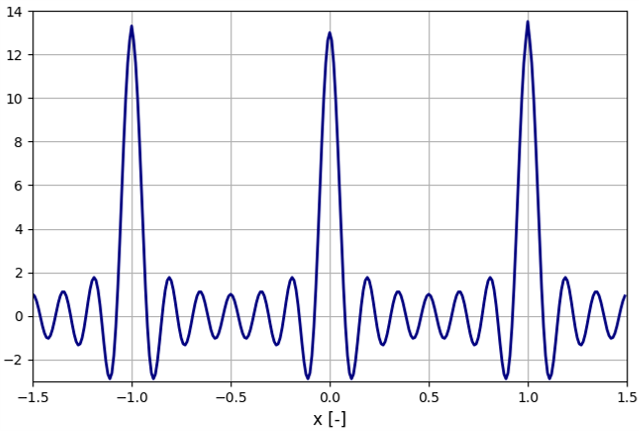
\includegraphics[width=8cm]{fig4.png}
\caption{$n=6$、$T=1$のときのディリクレカーネル}
\end{center}
\end{figure}

\subsubsection{フーリエ級数の理論}
\begin{itembox}[l]{定理2.1}
$f(t)$は周期$T$の周期関数であり、かつ区分的に滑らかな実関数であるとする。$f(t)$の複素フーリエ係数を$c_n$としたとき、$\sum_{n =-\infty}^\infty c_n e^{in\omega_0t}=(f(t+)+f(t-))/2$が成立する。
\end{itembox}
{\bf 証明}:フーリエ係数に関する部分和を$s_n(t)=\sum_{k=-n}^nc_ke^{ik\omega_0t}$と定義する。これは
\begin{equation}
s_n(t)=\sum_{k=-n}^n\left(\frac{1}{T}\int_{-T/2}^{T/2}f(u)e^{-ik\omega_0u}du\right)e^{ik\omega_0t}=\frac{1}{T}\int_{-T/2}^{T/2}f(u)\sum_{k=-n}^ne^{-ik\omega_0(u-t)}du \notag
\end{equation}
と書き表すこともできる。そこで$x=u-t$と定義すれば、上式は更に
\begin{equation}
s_n(t)=\frac{1}{T}\int_{-T/2-t}^{T/2-t}f(x+t)\sum_{k=-n}^ne^{-ik\omega_0x}dx=\frac{1}{T}\int_{-T/2}^{T/2}f(x+t)D_n(x)dx \notag
\end{equation}
と書き直される。$n \to \infty$としたとき、$s_n(t)$は正に複素フーリエ級数となるため、上式の最右辺が$(f(t+)+f(t-))/2$と等しいことを確かめれば本定理の証明をしたことになる。\par
ディリクレカーネルは偶関数であることを思い出すと、
\begin{equation}
\begin{array}{ll}
s_n(t) & = \frac{1}{T}\int_{-T/2}^{0}f(x+t)D_n(x)dx+\frac{1}{T}\int_{0}^{T/2}f(x+t)D_n(x)dx \\
& =\frac{1}{T}\int_{0}^{T/2}f(t-x)D_n(-x)dx+\frac{1}{T}\int_{0}^{T/2}f(t+x)D_n(x)dx \\
& =\frac{1}{T}\int_{0}^{T/2}(f(t+x)+f(t-x))D_n(x)dx
\end{array}\notag
\end{equation}
が成り立つと分かる。ここから更に
\begin{equation}
s_n(t)=\frac{1}{T}\int_{0}^{T/2}(f(t+x)-f(t+)+f(t-x)-f(t-))D_n(x)dx+\frac{1}{T}\int_{0}^{T/2}(f(t+)+f(t-))D_n(x)dx \notag
\end{equation}
なる式変形を施す。式(6)によれば右辺第二項は$(f(+)+f(t-))/2$に等しい。従って$n \to \infty$において右辺第一項がゼロとなることを確認できれば、本定理は証明できたことになる。$n \to \infty$の場合、ピーク以外のディリクレカーネルはゼロになるため、確かに第一項はゼロになりそうである。本資料ではこれで証明が完了したことにする。\qed \par
本定理はフーリエ級数に関して重要なことを教えてくれている。まず、区分的に滑らかな関数に関するフーリエ級数は収束する。また、連続である$t$(つまり$f(t)=f(t+)=f(t-)$を満たす$t$)において、フーリエ級数と元の関数値は一致する。\par
一方で不連続な点$t$の場合、フーリエ級数は元の関数の左右の平均、つまり$(f(t+)+f(t-))/2$と一致する。これは逆にフーリエ級数の値が$f(t)$に依存しないという点も面白い。例えば図5のようなステップ関数に関して不連続点の値が何であったとしても、その違いはフーリエ級数の結果に影響を与えない。

\begin{figure}[b]
\begin{center}
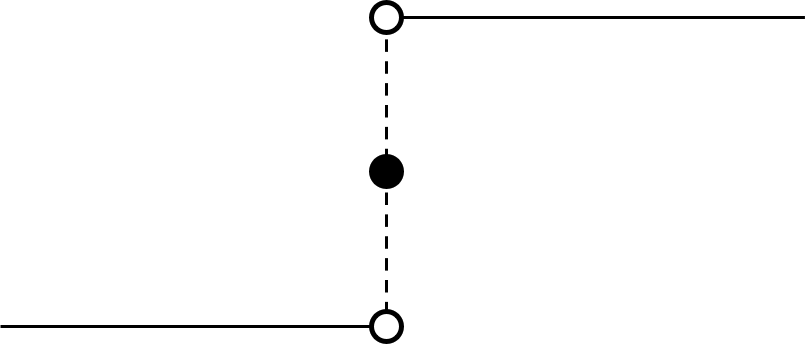
\includegraphics[width=5cm]{fig5.png}
\caption{不連続点を有する関数の例。不連続点におけるフーリエ級数の結果は、その点の関数値(図中黒丸)の値に依存しない。}
\end{center}
\end{figure}

\begin{itembox}[l]{定理2.2}
$f(t)$と$g(t)$は周期$T$の周期関数であり、かつ区分的に滑らかな実関数だとする。また$f(t)$に対応する複素フーリエ係数を$f_n$、$g(t)$に対応する複素フーリエ級数を$g_n$とする。任意の$n$に対して$f_n=g_n$であるとき、任意の連続点$t$において$f(t)=g(t)$が成立する。
\end{itembox}

\subsubsection{積と畳み込み積について}
\begin{itembox}[l]{命題2.6}
周期$T$の周期関数かつ区分的に滑らかな関数として$f(t)$と$g(t)$を考える。また、それぞれの複素フーリエ係数を$f_n$及び$g_n$とする。このとき、関数$h(t)=f(t)g(t)$も周期$T$の周期関数かつ区分的に滑らかな関数であるが、その複素フーリエ係数は$h_n=\sum_{k=-\infty}^\infty f_kg_{n-k}$となる。
\end{itembox}
{\bf 証明}:まず初めに
\begin{equation}
h_n=\int_{-T/2}^{T/2}f(t)g(t)e^{-in\omega_0t}dt \notag
\end{equation}
が言えるが、$f(t)$の部分を
\begin{equation}
h_n=\int_{-T/2}^{T/2}\sum_{k=-\infty}^\infty f_ke^{ik\omega_0t} g(t)e^{-in\omega_0t}dt \notag
\end{equation}
とのように書き換えても良い(連続な位置$t$であればこの書き換えに問題がないことは前項の通りである。また、不連続な点$t$でもそこの$f(t)$の値が積分に影響を与えることはない)。すると
\begin{equation}
h_n=\sum_{k=-\infty}^\infty f_k\int_{-T/2}^{T/2}g(t)e^{-i(n-k)\omega_0t}dt=\sum_{k=-\infty}^\infty f_kg_{n-k} \notag
\end{equation}
が得られるため本命題は正しい。\qed \par
命題2.4でベッセルの不等式を紹介したが、命題2.6を用いれば区分的に滑らかな関数なら等式が成立する。これは、関数$h(t)=f(t)f(t)$としたときの$h(0)$に関して
\begin{equation}
h_0=\sum_{k=-\infty}^\infty f_kf_{-k}=\sum_{k=-\infty}^\infty f_k\overline{f_k}=\sum_{k=-\infty}^\infty |f_k|^2=\frac{1}{T}\int_{-T/2}^{T/2}|f(t)|^2dt \notag
\end{equation}
が成立することより明かであろう。信号処理の分野において、信号$f(t)$に対する$P(t)=|f(t)|^2$なる関数は一般的にパワーと呼ばれており、重要な意味を持つ。そのため$P(t)$に関するフーリエ係数が$|f_n|^2$のように簡単に求まるということは有益な特性と言えよう。以下はより一般的な定理である。
\begin{itembox}[l]{定理2.3}
周期$T$の周期関数かつ区分的に滑らかな関数として$f(t)$と$g(t)$を考える。また、それぞれの複素フーリエ係数を$f_n$及び$g_n$とする。このとき、以下の等式が成立する(パーセバルの等式)。
\begin{equation}
\frac{1}{T}\int_{-T/2}^{T/2}f(t)\overline{g(t)}dt=\sum_{n=-\infty}^\infty f_n\overline{g_n} \notag
\end{equation}
\end{itembox}

\begin{tcolorbox}[title=畳み込み積分]
周期$T$の周期関数かつ区分的に滑らかな関数として$f(t)$と$g(t)$を考える。このとき、下記のように定義される新たな関数のことを、$f$と$g$の畳み込み積分と言い、$(f*g)(t)$と表記する。
\begin{equation}
(f*g)(t)=\frac{1}{T}\int_{-T/2}^{T/2}f(t-\tau)g(\tau)d\tau \notag
\end{equation}
\end{tcolorbox}
$(f*g)(t)$も周期$T$の周期関数であることは
\begin{equation}
(f*g)(t+kT)=\frac{1}{T}\int_{-T/2}^{T/2}f(t+kT-\tau)g(\tau) d\tau=\frac{1}{T}\int_{-T/2}^{T/2}f(t-\tau)g(\tau)d\tau=(f*g)(t) \notag
\end{equation}
より確認できる。
\begin{itembox}[l]{命題2.7}
周期$T$の周期関数かつ区分的に滑らかな関数として$f(t)$と$g(t)$を考える。また、それぞれの複素フーリエ係数を$f_n$及び$g_n$とする。このとき、$(f*g)(t)$の複素フーリエ係数は$f_ng_n$となる。
\end{itembox}
{\bf 証明}:
\begin{equation}
\begin{array}{ll}
(f*g)_n & =\frac{1}{T}\int_{-T/2}^{T/2}\left(\frac{1}{T}\int_{-T/2}^{T/2}f(t-\tau)g(\tau)d\tau \right)e^{-in\omega_0t}dt \\
&=\frac{1}{T}\int_{-T/2}^{T/2}\left(\frac{1}{T}\int_{-T/2}^{T/2}f(t-\tau)e^{-in\omega_0(t-\tau)}dt \right)g(t-\tau)e^{-in\omega_0\tau}d\tau \\
& =f_ng_n
\end{array}\notag
\end{equation}
より明らか。\qed

\subsubsection{積分について}
\begin{itembox}[l]{補題2.1}
周期$T$の周期関数かつ区分的に滑らかな関数として$f(t)$を考える。$f(t)$を
\begin{equation}
h(t)=\int_{-T/2}^tf(\tau)d\tau
\end{equation}
のように積分した関数も周期$T$の周期関数である場合かつそのときに限り、$f(t)$のフーリエ係数$c_n$のうち$c_0$はゼロである。
\end{itembox}
{\bf 証明}:$h(t)$に関して
\begin{equation}
h(t+T)=\int_{-T/2}^{t+T}f(\tau)d\tau=\int_{-T/2}^{T/2}f(\tau)d\tau+\int_{T/2}^{t+T}f(\tau)d\tau=\int_{-T/2}^{T/2}f(\tau)d\tau+\int_{-T/2}^tf(\tau)d\tau \notag
\end{equation}
が成り立つ。これが$h(t)$と等しいため、上式の最右辺第一項はゼロでなければならない。これは正に$c_0$であるため、本補題は正しい。\qed
\begin{itembox}[l]{命題2.8}
周期$T$の周期関数かつ区分的に滑らかな関数として$f(t)$を考える。また$f(t)$のフーリエ係数を$c_n$で書き表し、$c_0=0$とする。このとき、式(7)の関数$h(t)$は自身のフーリエ級数と等しい。つまり$h(t)0=\sum_{n=-\infty}^\infty h_ne^{in\omega_0t}$が成立する。ここでフーリエ係数は
\begin{equation}
h_n=
\left\{
\begin{array}{ll}
c_n/(in\omega_0) & n \neq 0 \\
-\sum_{n \neq 0}(-1)^nc_n/(in\omega_0) & n=0
\end{array}
\right. \notag
\end{equation}
である。 
\end{itembox}
{\bf 証明}:まず初めに
\begin{equation}
g(\tau)=
\left\{
\begin{array}{ll}
1 & -T/2 \leq \tau \leq t \\
0 & t < \tau \leq T/2
\end{array}\right. \notag
\end{equation}
なる関数を定義する。すると式(7)の$h(t)$は
\begin{equation}
h(t)=\int_{-T/2}^{T/2}f(\tau)\overline{g(\tau)}d\tau=T\sum_{n=-\infty}^\infty c_n\overline{g_n}=\sum_{n=-\infty}^\infty c_n \overline{\int_{-T/2}^{T/2}g(\tau)e^{-in\omega_0\tau}d\tau}=\sum_{n=-\infty}^\infty c_n\int_{-T/2}^te^{in\omega_0\tau}d\tau \notag
\end{equation}
のように定義することもできる(定理2.3)。いま$c_0=0$なので
\begin{equation}
h(t)=\sum_{n \neq 0}c_n\int_{-T/2}^te^{in\omega_0\tau}d\tau=\sum_{n \neq 0}\frac{c_n}{in\omega_0}e^{in\omega_0t}-\sum_{n \neq 0} \frac{c_n(-1)^n}{in\omega_0} \notag
\end{equation}
が得られる。最右辺の第二項は$h_0$に相当し、第一項はそれぞれ$h_n$に相当する。従って本命題は正しい。\qed

\subsubsection{微分について}
\begin{itembox}[l]{命題2.9}
周期$T$の周期関数かつ区分的に滑らかな関数として$f(t)$を考える。また$f(t)$のフーリエ係数を$c_n$で書き表すとしたとき、以下の等式が成立する。
\begin{equation}
\frac{1}{2}(f'(t+)+f'(t-))=\sum_{n=-\infty}^\infty in\omega_0c_ne^{in\omega_0t} \notag
\end{equation}
\end{itembox}
{\bf 証明}:$f'(t)$のフーリエ係数を$c'_n$としたとき、
\begin{equation}
c_n'=\int_{-T/2}^{T/2}f'(t)e^{-in\omega_0t}dt=\frac{1}{T}\left[ f(t)e^{-in\omega_0t} \right]_{-T/2}^{T/2}+in\omega_0\frac{1}{T}\int_{-T/2}^{T/2}f'(t)e^{-in\omega_0t}dt \notag
\end{equation}
が成立する。$f(t)$は周期関数であるため、最右辺第一項はゼロになる。従って$c_n'=in\omega_0c_n$の関係が得られる。いま、$f(t)$は区分的に滑らかなので、$f'(t)$は区分的連続だと言える。従って本命題は正しい。

\subsection{周期的入力に対するLTCシステムの応答}
本項ではフーリエ級数の応用例として、周期的入力に対するLTCシステムの応答を考える。物理で扱う多くの入力は実関数だが、複素フーリエ級数で考えるために入力を$e^{i\omega t}$のように考えることにする。\par
入力$u(t)$は区分的に滑らかであり、
\begin{equation}
u(t)=\sum_{n=-\infty}^\infty u_n e^{in\omega_0t} \notag
\end{equation}
のようにフーリエ級数と一致すると仮定する。ここで$\omega_0$は基本周波数であり、$u(t)$の周期を$T$としたとき$\omega_0=2\pi/T$である。LTCシステムの応答を$H(\omega)$としたとき、定理1.1より出力$y(t)$は
\begin{equation}
y(t)=\sum_{n=-\infty}^\infty u_nH(n\omega_0) e^{in\omega_0t} \notag
\end{equation}
となる。\par
本資料の冒頭で述べた通り、システムを偏微分方程式で表すことが多い。特にLTCシステムの場合、係数が一定の偏微分方程式
\begin{equation}
a_m\frac{d^my}{dt^m}+a_{m-1}\frac{d^{m-1}y}{dt^{m-1}}+...+a_1\frac{dy}{dt}+a_0y=b_n\frac{d^nu}{dt^n}+b_{n-1}\frac{d^{n-1}u}{dt^{n-1}}+...+b_1\frac{du}{dt}+b_0u
\end{equation}
で表すことができる。ここで$a_m\neq 0$および$b_n \neq 0$である。また物理の問題においては$n \leq m$に限定することができる。このLTCシステムに対応する偏微分方程式に対して、
\begin{equation}
\begin{array}{l}
A(s)=a_ms^m+a_{m-1}s^{m-1}+...+a_1s+a_0 \\
B(s)=b_ns^n+b_{n-1}s^{n-1}+...+b_1s+b_0
\end{array}
\end{equation}
の複素多項式を考えよう。なお$A(s)$のことを特別に固有多項式と言う。以下は応答に関する定理である。
\begin{itembox}[l]{定理2.4}
式(8)の偏微分方程式に対応するLTCシステムを考える。$A(i\omega)\neq 0$を満たす任意の$\omega$において、LTCシステムの応答は$H(\omega)=B(i\omega)/A(i\omega)$となる。
\end{itembox}
{\bf 証明}:入力が$e^{i\omega t}$のとき、出力は定義より$H(\omega)e^{i\omega t}$となる。従って式(8)より
\begin{equation}
H(\omega)\left(a_m\frac{d^me^{i\omega t}}{dt^m}+a_{m-1}\frac{d^{m-1}e^{i\omega t}}{dt^{m-1}}+...+a_1\frac{de^{i\omega t}}{dt}+a_0e^{i\omega t}\right)=b_n\frac{d^ne^{i\omega t}}{dt^n}+b_{n-1}\frac{d^{n-1}e^{i\omega t}}{dt^{n-1}}+...+b_1\frac{de^{i\omega t}}{dt}+b_0e^{i\omega t} \notag
\end{equation}
が成り立つ。各項を微分していけば$H(\omega)=B(i\omega)/A(i\omega)$が実際に得られるため、本定理は正しい。\qed \par
入力$u(t)$が所与のとき、式(8)の右辺も所与であるため出力$y(t)$も求まる。ただし、出力が一意に定まるかどうかは分からない。式(8)の左辺に関する偏微分方程式
\begin{equation}
a_m\frac{d^mx}{dt^m}+a_{m-1}\frac{d^{m-1}x}{dt^{m-1}}+...+a_1\frac{dx}{dt}+a_0x=0
\end{equation}
とその解$x(t)$を考える。式(8)に対する式(10)を同次微分方程式と言い、その解を特別に固有関数と言う。固有関数は$u(t)=0$、つまり入力信号がゼロのときの出力と見ることができる。また、$x(t)=0$も式(10)の解だが、それはトリビアルな解だとし特別考察することはない。さて、「出力が一意に定まるか分からない」と先程述べたが、それは$y(t)$が式(8)を満たすならば、$y(t)+x(t)$も式(8)を満たすためである。\par
固有関数について更に議論していこう。式(10)に対して$x=e^{st}$の場合を考える(式(10)より一般性を欠くことなく大きさ1の複素数で考えてもよい)。すると式(10)は$a_ms^m+a_{m-1}s^{m-1}+...+a_1s+a_0=0$に書き換えられる。これは正に式(9)の固有多項式である。従って$A(s)=0$を満たすような$s \in \mathbb{C}$が分かれば、$e^{st}$は固有関数ということも分かる。代数学の定理より、$A(s)=0$は$m$個の解を有する。$m$個の解をそれぞれ$\{ s_1,...,s_m \}$としたとき、これらの線形結合も式(10)を満たす。従って式(10)の解のベクトル空間を考えたとき、集合$\{ s_1,...,s_m \}$は正に基底だと言える。\par
では次に、固有多項式が虚軸に解を持つとき、つまり$A(i\omega)=0$となるような$\omega \in \mathbb{R}$が存在するときを考えよう。このような$\omega$を固有周波数と言う。このとき、$x=e^{i\omega t}$は式(10)を満たすので、「固有多項式が純虚数な解を有するとき、周期$T=2\pi/|\omega|$の固有関数が存在する」と言える。もしも入力$u(t)$を$e^{i\omega t}$としたとき、出力も同じ周期$T$の関数となるが、固有関数がある分一意に定まらない。それどころか、定理2.4より発散することが分かっている(つまり安定システムではない)。このような発散現象を物理では共鳴と言う。

\section{フーリエ積分}
前章では周期関数のみを扱い、それに対するフーリエ級数を議論した。いくつかの条件を満たす関数が三角関数系の線形結合で表せるという点は興味深い一方、実用上では非周期関数を扱わなければならないことも多い。本章では非周期関数における前章同様の理論として、フーリエ積分を議論する。ただし、これも前章と同様に、いきなり数学的に厳密な議論をしてしまっては消化不良を起こすため、まずは数学的厳密さを大胆に欠いて大まかな理解に挑戦する。

\subsection{フーリエ積分の基礎}
いま、実数域全体で定義された非周期関数$f:\mathbb{R} \to \mathbb{R}$を考える(対象の関数が実数域全体で定義されていなかった場合、定義されていない値$t$では$f(t)=0$として拡張することが実用上多い)。直感的な説明だが、非周期関数は周期$T \to \infty$な周期関数と考えることもできる。従って関数が区分的に滑らかである場合、フーリエ級数より
\begin{equation}
f(t)={\rm lim}_{T\to \infty}\sum_{n=-\infty}^\infty \frac{1}{T}\int_{-T/2}^{T/2}f(\tau)e^{in\Delta \omega (t-\tau)}d\tau
\end{equation}
となる。ここで$\Delta \omega$は基本周波数$2\pi/T$だが$\Delta \omega \to 0$であるため、これまでと表記を変えた。さて、
\begin{equation}
G(\omega)=\int_{-\infty}^\infty f(\tau)e^{i\omega(t-\tau)}d\tau \notag
\end{equation}
なる関数を定義したとき、
\begin{equation}
{\rm lim}_{\Delta \omega \to 0}\frac{1}{2\pi}\sum_{n=-\infty}^\infty G(n\Delta \omega)\cdot \Delta \omega={\rm lim}_{\Delta \omega \to 0} \frac{\Delta \omega}{2\pi}\sum_{n=-\infty}^\infty\int_{-\infty}^\infty f(\tau)e^{in\Delta \omega(t-\tau)}d\tau \notag
\end{equation}
なる関係が得られる。左辺はリーマン和のようなもので、積分で書くこともできる。従って、上式より
\begin{equation}
f(t)=\frac{1}{2\pi}\int_{-\infty}^{\infty}\left( \int_{-\infty}^\infty f(\tau)e^{-i\omega \tau}d\tau \right)e^{i\omega t}d\omega \notag
\end{equation}
なる関係が得られる。積分と和という違いはあれど、これはフーリエ級数における式と似ている。「フーリエ積分では基本周波数に相当するものがゼロに近づいたため積分化した」と考えればよい。右辺のことをフーリエ積分と言う。また、フーリエ係数に相当するものをフーリエ積分ではフーリエ変換と言う。
\begin{tcolorbox}[title=フーリエ変換]
関数$f$に対して$F(\omega)=\int_{-\infty}^\infty f(t)e^{-i\omega t}dt$が存在するとき、これをフーリエ変換と言う。
\end{tcolorbox}
\begin{tcolorbox}[title=絶対積分可能]
関数$f:\mathbb{R} \to \mathbb{R}$に対して$\int_{-\infty}^{\infty}|f(t)|dt$が存在するとき、関数$f$は$\mathbb{R}$上で絶対積分可能であると言う。
\end{tcolorbox}
定義より
\begin{equation}
|F(\omega)|=|\int_{-\infty}^\infty f(t)e^{-i\omega t}dt| \leq \int_{-\infty}^\infty |f(t)||e^{-i\omega t}|dt=\int_{-\infty}^\infty |f(t)|dt \notag
\end{equation}
であるため、フーリエ変換が存在するならば関数$f$は絶対積分可能だと言えそうである(厳密な議論を私は知らない)。\par
フーリエ級数との相似性を考えれば、
\begin{equation}
f(t)=\frac{1}{2\pi}\int_{-\infty}^\infty F(\omega)e^{i\omega t}d\omega \notag
\end{equation}
が成立しそうである。確かに多くの場合成り立つが、そうでないときもある。例えば$f(t)$が絶対積分可能であったとしても、$F(\omega)$がそうである保証はなく、右辺の結果が存在しないこともある。また、たとえ存在したとしても、それが$f(t)$に一致する保証は議論されていない。その辺りは次節で触れることにしよう。

\subsubsection{フーリエ変換の性質}
\begin{itembox}[l]{命題3.1}
フーリエ変換は線形性を有する。関数$f(t)$および$g(t)$と、それぞれのフーリエ変換$F(\omega)$および$G(\omega)$を考える。このとき$af(t)+bg(t)$のフーリエ変換は$aF(\omega)+bG(\omega)$となる。
\end{itembox}
\begin{itembox}[l]{命題3.2}
関数$f(t)$とそのフーリエ変換$F(\omega)$を考える。$\overline{f(t)}$のフーリエ変換は$\overline{F(-\omega)}$である。
\end{itembox}
{\bf 証明}:定義より
\begin{equation}
\int_{-\infty}^\infty \overline{f(t)}e^{-i\omega t}d\omega=\overline{\int_{-\infty}^\infty \overline{f(t)}e^{i\omega t}d\omega}=\overline{F(-\omega)} \notag
\end{equation}
であるため明らか。\qed
\begin{itembox}[l]{命題3.3}
関数$f(t)$とそのフーリエ変換$F(\omega)$を考える。$f(t-a)$のフーリエ変換は$e-{-i\omega a}F(\omega)$である。
\end{itembox}
{\bf 証明}:定義より
\begin{equation}
\int_{-\infty}^\infty f(t-a)e^{-i\omega (t-a)}e^{-i\omega a}d\omega=e^{-i\omega a}F(\omega) \notag
\end{equation}
であるため明らか。\qed
\begin{itembox}[l]{命題3.4}
関数$f(t)$とそのフーリエ変換$F(\omega)$を考える。$e^{iat}f(t)$のフーリエ変換は$F(\omega-a)$である。
\end{itembox}\par
命題3.4より、$f(t){\rm cos}at$のフーリエ変換は$\{F(\omega-a)+F(\omega+a)\}/2$だということも分かる。
\begin{itembox}[l]{命題3.5}
関数$f(t)$とそのフーリエ変換$F(\omega)$を考える。ゼロ以外の任意の実数$c$に対して、$f(ct)$のフーリエ変換は$F(c^{-1}\omega)/|c|$となる。
\end{itembox}
{\bf 証明}:まず初めに$c>0$の場合を考える。定義より
\begin{equation}
\int_{-\infty}^\infty f(ct)e^{-i\omega t}dt=\frac{1}{c}\int_{-\infty}^\infty f(\tau)e^{-i\omega \tau/c}d\tau=F(c^{-1}\omega)/c \notag
\end{equation}
となるため、本命題と合致する。$c<0$の場合も同様に確かめられる。\qed
\begin{itembox}[l]{命題3.6}
関数$f(t)$が偶関数であるとき、$f(t)$のフーリエ変換は$F(\omega)=2\int_0^\infty f(t)\cos \omega tdt$である。
\end{itembox}
命題3.6は偶関数の定義より明らかである。一般的に、$F_c(\omega)=\int_0^\infty f(t)\cos \omega tdt$のことをフーリエコサイン変換と呼ぶ。命題3.5より、$F(-\omega)=F(\omega)$であるため、$f(t)$が偶関数ならそのフーリエ変換も偶関数であることが解る。また、$f(t)$が実関数ならば、本命題より$F(\omega)$も実関数だと解る。\par
\begin{itembox}[l]{命題3.7}
関数$f(t)$が奇関数であるとき、$f(t)$のフーリエ変換は$F(\omega)=-2i\int_0^\infty f(t)\sin \omega tdt$である。
\end{itembox}
命題3.6は偶関数の定義より明らかである。一般的に、$F_s(\omega)=\int_0^\infty f(t)\sin \omega tdt$のことをフーリエサイン変換と呼ぶ。命題3.5より、$F(-\omega)=-F(\omega)$であるため、$f(t)$が奇関数ならそのフーリエ変換も奇関数であることが解る。また、$f(t)$が実関数ならば、本命題より$F(\omega)$は純虚数の関数だと解る。\par

\begin{itembox}[l]{命題3.8(自己双対性)}
区分的に滑らかで、絶対積分可能な2つの関数$f(t)$と$g(t)$を考える。それぞれのフーリエ変換を$F(\omega)$及び$G(\omega)$とする。このとき、以下の等式が成立する。
\begin{equation}
\int_{-\infty}^\infty f(x)G(x)dx=\int_{-\infty}^\infty F(x)g(x)dx \notag
\end{equation}
\end{itembox}
{\bf 証明}:定義より
\begin{equation}
\int_{-\infty}^\infty f(x)G(x)dx=\int_{-\infty}^\infty f(x)\left(\int_{-\infty}^\infty g(y)e^{-ixy}dy\right)dx=\int_{-\infty}^\infty g(y)\left(\int_{-\infty}^\infty f(x)e^{-ixy}dx\right)dy=\int_{-\infty}^\infty F(x)g(x)dx \notag
\end{equation}
だと解るので、本命題は正しい。\qed
\begin{itembox}[l]{命題3.9}
$f(t)$は滑らかな関数であり、${\rm lim}_{t \to \pm \infty}f(t)=0$であるとする。$f(t)$のフーリエ変換を$F(\omega)$としたとき、$f'(t)$のフーリエ変換は$i\omega F(\omega)$である。
\end{itembox}
{\bf 証明:}定義より、
\begin{equation}
\int_{-\infty}^\infty f'(t)e^{-i\omega t}dt=\left[f(t)e^{-i\omega t}\right]_{-\infty}^\infty + i\omega \int_{-\infty}^\infty f(t)e^{-i\omega t}dt=i\omega F(\omega) \notag
\end{equation}
であるから、本命題は正しい。

\begin{itembox}[l]{命題3.10}
$f(t)$は絶対積分可能な関数であり、そのフーリエ変換を$F(\omega)$と書き表す。$tf(t)$も絶対積分可能であるとき、$F(\omega)$は微分可能であり、$F'(\omega)=(F~itf(t))(\omega)$である。
\end{itembox}
{\bf 証明}:$F(\omega)$に関して
\begin{equation}
{\lim}_{h \to 0}\frac{F(\omega+h)-F(\omega)}{h}={\rm lim}_{h \to 0}\int_{-\infty}^\infty f(t)\frac{e^{-i(\omega+h)t}-e^{-i\omega t}}{h}dt={\rm lim}_{h \to 0}\int_{-\infty}^\infty f(t)e^{-i\omega t}\frac{e^{-iht}-1}{h}dt \notag
\end{equation}
を考える。証明は省くが、${\rm lim}$と積分は順序交換可能であり、
\begin{equation}
{\rm lim}_{h \to 0}\frac{e^{-iht}-1}{h}={\rm lim}_{h \to 0}\left( \frac{\cot ht-1}{h}-i\frac{\sin ht}{h} \right)=-it \notag
\end{equation}
であるため、
\begin{equation}
{\lim}_{h \to 0}\frac{F(\omega+h)-F(\omega)}{h}=\int_{-\infty}^\infty (-itf(t))e^{-i\omega t}dt \notag
\end{equation}
が得られる。いま$tf(t)$は絶対積分可能であるため、上式右辺は確かに求まる。従って$F(\omega)$は微分可能であり、導関数も本命題の通りである。\qed

\begin{itembox}[l]{命題3.11}
$f(t)$は${\rm lim}_{t \to \infty}\int_{-\infty}^tf(\tau)d\tau=0$を満たす連続で絶対積分可能な関数だとする。そのフーリエ変換を$F(\omega)$としたとき、$\int_{-\infty}^tf(\tau)d\tau$のフーリエ変換は$F(\omega)/i\omega$である(ただし$\omega \neq 0$)。
\end{itembox}
{\bf 証明}:$g(t)=\int_{-\infty}^tf(\tau)d\tau$としたとき、$g'(t)=f(t)$である。従って$g'(t)$のフーリエ変換が$F(\omega)$である訳だから、命題3.9より明らか。\qed

\begin{tcolorbox}[title=急減小関数]
任意の$k \in \mathbb{N}$に対して、$k$回導関数が存在する関数$f:\mathbb{R} \to \mathbb{C}$のすべての集合を$\mathbb{C}^\infty(\mathbb{R})$と書く。$f \in \mathbb{C}^\infty(\mathbb{R})$が以下の条件を満たすとき、急減小関数と言う。
\begin{itemize}
\item 任意の$m, n \in \mathbb{N}$に対して、$|t^nf^{(m)}(t)|<M$を満たす$M$が存在する。
\end{itemize}
\end{tcolorbox}
当然ながら$M$の値は$n$と$m$に依存する。上記の条件を満たすとき、$m=0$ならば$|f(t)|<M|t|^{-n}$と書ける。当然ながら${\rm lim}_{t \to \pm \infty}|t|^{-n}=0$であり、(抽象的な言い方だが)$|t|^{-n}$は急激な現象を見せる($n \in \mathbb{N}$であることに注意)。それゆえ$f(t)$は急減小だと言われている次第である。\par
\begin{itembox}[l]{定理3.1}
急減小関数の集合$\mathcal{S}$はベクトル空間(シュワルツ空間と言う)である。
\end{itembox}
{\bf 証明}:任意の$c \in \mathbb{C}$に対して、$f \in \mathcal{S}$ならば$cf \in \mathcal{S}$であることは明らか。同様に、$f, g \in \mathcal{S}$について
\begin{equation}
|t^n(f+g)^{(m)}(t)|=|t^nf^{(m)}(t)+t^ng^{(m)}(t)| \leq |t^nf^{(m)}(t)| + |t^ng^{(m)}(t)| \notag
\end{equation}
であるため、$f+g \in \mathcal{S}$。従って本定理は正しい。\qed

\begin{itembox}[l]{命題3.12}
シュワルツ空間はフーリエ変換に対して不変である。つまり、関数$f$のフーリエ変換が$F$であるとき、$f \in \mathcal{S}$ならば$F \in \mathcal{S}$である。
\end{itembox}

\begin{tcolorbox}[title=畳み込み積分]
2つの関数$f$および$g$に対して、畳み込み積分$f*g$を
\begin{equation}
(f*g)(t)=\int_{-\infty}^\infty f(\tau)g(t-\tau)d\tau \notag
\end{equation}
と定義する(ただし上式の積分が存在する場合に限る)。
\end{tcolorbox}
畳み込み積分は既に2章でも紹介したが、これは非周期関数における定義だと考えればよい。\par
一方の関数(例えば$f$)が絶対積分可能で、他方の関数(例えば$g(t)\leq M$)が有界であるとき、畳み込み積分は存在する。これは、
\begin{equation}
|(f*g)(t)|=\left|\int_{-\infty}^\infty f(\tau)g(t-\tau)d\tau \right| \leq \int_{-\infty}^\infty |f(\tau)g(t-\tau)|d\tau \leq M\int_{-\infty}^\infty |f(\tau)|d\tau \notag
\end{equation}
から確認できる。

\begin{itembox}[l]{命題3.13}
$(f*g)(t)=(g*f)(t)$が成り立つ。
\end{itembox}
\begin{itembox}[l]{定理3.2}
区分的に滑らかで、有界かつ絶対積分可能な関数$f(t), g(t)$を考える。それぞれのフーリエ変換を$F(\omega), G(\omega)$とする。このとき、$(f*g)$のフーリエ変換は$F(\omega)G(\omega)$である。
\end{itembox}
前提より、
\begin{equation}
\int_{-\infty}^\infty |(f*g)(t)|dt \leq \int_{-\infty}^\infty \left(\int_{-\infty}^\infty |f(\tau)g(t-\tau)|dt \right)d\tau = \int_{-\infty}|f(\tau)|d\tau \int_{-\infty}^\infty |g(u)|du < \infty \notag
\end{equation}
であるから(ここで$u=t-\tau$)、$f*g$は絶対積分可能である。したがって$f*g$のフーリエ変換は存在する。定義より、
\begin{equation}
\mathcal{F}(f*g)(\omega)=\int_{-\infty}^\infty f(\tau)e^{-i\omega \tau}\left( \int_{-\infty}^\infty g(t-\tau)e^{-i\omega(t-\tau)}dt \right) d\tau=F(\omega)G(\omega) \notag
\end{equation}
であるから、本命題は正しい。

\begin{itembox}[l]{命題3.14}
区分的に連続で絶対積分可能である実関数$f$を考える。$f$のフーリエ変換を$F$としたとき、以下の等式が成立する。
\begin{equation}
{\rm lim}_{\omega \to \pm \infty} F(\omega)={\rm lim}_{\omega \to \pm \infty}\int_{-\infty}^\infty f(t)e^{-i\omega t}dt=0 \notag
\end{equation}
\end{itembox}
{\bf 証明}:$f$は絶対積分可能であるため、任意の正の実数$\epsilon$に対して、
\begin{equation}
\int_{T}^\infty |f(t)|dt + \int_{-\infty}^{-T}|f(t)|dt<\frac{\epsilon}{2} \notag
\end{equation}
を満たす正の実数$T \in \mathbb{R}$が存在する。また、命題2.5より、正の実数$G$について、$|\omega|>G$を満たす任意の$\omega$で
\begin{equation}
\left|\int_{-T}^T f(t)e^{-i\omega t} dt\right|<\frac{\epsilon}{2} \notag
\end{equation}
を満たすような$G$が存在する。よって三角不等式より
\begin{equation}
\left| \int_{-\infty}^\infty f(t)e^{-i\omega t}dt \right| \leq \int_{T}^\infty |f(t)|dt + \int_{-\infty}^{-T}|f(t)|dt + \left|\int_{-T}^T f(t)e^{-i\omega t} dt\right| < \epsilon \notag
\end{equation}
が成立する。よって本命題は正しい。\qed \par
本命題はフーリエ級数に関する命題2.5の、フーリエ積分におけるものと言える。


\subsection{フーリエ積分の理論}
関数$f$とそのフーリエ変換$F$について、
\begin{equation}
f(t)=\frac{1}{2\pi}\int_{-\infty}^\infty F(\omega)e^{i\omega t}d\omega \notag
\end{equation}
が成立するようなことを前節で触れた。これはフーリエ級数との類似性を考えれば納得感があり、実際に$f$がいくつかの条件を満たせば成立する。本書ではこの等式を直感的に説明し、厳密な証明は他書に譲ることにした。\par
それではまず右辺から観察することにしよう。右辺は
\begin{equation}
{\rm lim}_{A \to \infty}\frac{1}{2\pi}\int_{-A}^A F(\omega)e^{i\omega t}d\omega \notag
\end{equation}
と書き換えても差支えない。これは
\begin{equation}
\frac{1}{2\pi}\int_{-A}^A F(\omega)e^{i\omega t}d\omega=\frac{1}{2\pi}\int_{-A}^A \left(\int_{-\infty}^{\infty} f(s)e^{-i\omega s}ds \right)e^{i\omega t}d\omega=\frac{1}{2\pi}\int_{-\infty}^\infty f(s) \left(\int_{-A}^A e^{i\omega (t-s)}d\omega \right)ds = \frac{1}{\pi}\int_{-\infty}^\infty f(t-\tau)\frac{\sin A\tau}{\tau}d\tau \notag
\end{equation}
と書き換えることができる(ここで$\tau=t-s$)。関数$(\sin A\tau)/\tau$の特徴はフーリエ積分の直感的理解において重要で、$A$の増加と共にデルタ関数$\delta(\tau)$のようになる。そうなってくると、確かに$f(t)$と$F(\omega)$の関係性はなんとなく見えてくるだろう。証明は省くが、実際に
\begin{equation}
{\rm lim}_{A \to \infty}\frac{1}{\pi}\int_{-\infty}^\infty f(t-\tau)\frac{A\tau}{\tau}=\frac{1}{2}(f(t+)+f(t-)) \notag
\end{equation}
が成立することが解っている。以上より、フーリエ積分に関する重要な定理が得られる。
\begin{tcolorbox}[title=フーリエ積分]
区分的に滑らかかつ絶対積分可能な実関数$f$を考える。このフーリエ変換が$F$であるとすれば、以下の等式が成立する。
\begin{equation}
\frac{1}{2\pi}\int_{-\infty}^\infty F(\omega)e^{i\omega t}d\omega =\frac{1}{2}(f(t+)+f(t-))
\end{equation}
\end{tcolorbox}
不連続点$t$の関数値$f(t)$がフーリエ変換の結果に影響を与えないということはあれど、式(12)は$F$から$f$への変換と言える。それゆえこのような処理を一般的にフーリエ逆変換と言う。\par
フーリエ逆変換の計算は、$f$が偶関数もしくは奇関数の場合、フーリエコサイン変換及びフーリエサイン変換の結果を用いることでより簡易になる。例えば$f$が偶関数の場合、フーリエ逆変換は
\begin{equation}
\frac{2}{\pi}\int_0^\infty F_c(\omega)\cos \omega td\omega = \frac{1}{2}(f(t+)+f(t-)),~~~F_c(\omega)=\int_0^\infty f(t)\cos \omega tdt \notag
\end{equation}
のように書き表され、一方で$f$が奇関数の場合は
\begin{equation}
\frac{2}{\pi}\int_0^\infty F_s(\omega)\sin \omega td\omega = \frac{1}{2}(f(t+)+f(t-)),~~~F_s(\omega)=\int_0^\infty f(t)\sin \omega tdt \notag
\end{equation}
のようになる。

\end{document}

\subsection{分布}
\subsection{分布とフーリエ積分}
\section{ラプラス変換}






